Debido a la \textit{"intratabilidad"} del problema de la partición de un grafo, no existe un algoritmo concreto que permita obtener en tiempo polinómico una solución óptima a la partición de cualquier grafo. Es por ello que, los algoritmos codificados para este trabajo se basan en la metaheurística, con el objetivo de obtener soluciones de buena calidad en tiempos computacionales aceptables, a pesar de que los algoritmos metaheurísticos no garantizan que se vaya a obtener una solución óptima al problema, incluso podría suceder que no se obtenga ninguna solución. 

En el siguiente apartado se analizan los algoritmos Kernighan-Lin\cite{KernighanLin} (ver apartado \ref{Kernighan-Lin}), Specrtal Bisection (ver apartado \ref{Spectral-Bisection}) y Multilevel Spectral Bisection (ver apartado \ref{Multilevel-Spectral-Bisection}), tres algoritmos diseñados específicamente para la resolución del problema de la partición de grafos. Cualquiera de estos algoritmos proporciona una solución factible al problema, pudiendo ser esta óptima o no. Además de describir cada uno de los algoritmos detalladamente, las principales propiedades de cada uno de ellos, también se describirán algunos ejemplos.

\section{Kernighan-Lin}\label{Kernighan-Lin}

El algoritmo Kernighan-Lin\cite{KernighanLin}, a menudo abreviado como K-L, es uno de los primeros algoritmos de partición de grafos y fue desarrollado originalmente para optimizar la colocación de circuitos electrónicos en tarjetas de circuito impreso para minimizar el número de conexiones entre las tarjetas.

El algoritmo K-L no crea particiones, sino que las mejora iterativamente. La idea original era tomar una partición aleatoria y aplicarle Kernighan-Lin\cite{KernighanLin}. Esto se repetiría varias veces y se elegiría el mejor resultado. Mientras que para grafos pequeños esto ofrece resultados razonables, es bastante ineficiente para tamaños de problemas más grandes.

Decimos que es un algoritmo:

\begin{itemize}
	\setlength{\parskip}{0pt}
	\setlength{\itemsep}{0pt plus 1pt}
	\item \textbf{Iterativo}. Esto significa que el grafo inicialmente ya está particionado, pero la aplicación del algoritmo intentará mejorar u optimizar la partición inicial. 
	\item \textbf{Voraz}. Esto significa que el algoritmo hará cambios si hay un beneficio inmediato sin considerar otras formas posibles de obtener una solución óptima.
	\item \textbf{Determinista} porque se obtendrá el mismo resultado cada vez que se aplique el algoritmo. 
\end{itemize}

%Una aplicación importante del algoritmo es en los circuitos VLSI\cite{KernighanLin}\cite{Ravikumar}. Concretamente se usa para encontrar un número mínimo de conexiones entre particiones para mejorar la velocidad o disminuir el consumo de energía.

Hoy en día, el algoritmo se usa para mejorar las particiones encontradas por otros algoritmos. Como veremos, K-L tiene una visión algo \textit{"local"} del problema, tratando de mejorar las particiones mediante el intercambio de nodos vecinos. Por lo tanto, complementa muy bien los algoritmos que tienen una visión más \textit{"global"} del problema, pero tienden a ignorar las características locales. Un ejemplo de este tipo de algoritmos seria la partición espectral (ver sección \ref{Spectral-Bisection}).

C. Fiduccia y R. Mattheyses realizaron importantes avances prácticos en \cite{FiducciaMattheyses} quienes mejoraron el algoritmo de tal manera que una iteración se ejecuta en $O({n}^2)$ en lugar de $O({n}^2 \, log \, n)$.

\subsection{Descripción}

Ventajas:

\begin{itemize}
	\item El algoritmo es robusto.
\end{itemize}

Desventajas:

\begin{itemize}
	\item Los resultados son aleatorios porque el algoritmo comienza con una partición aleatoria.
	\item Computacionalmente es un algoritmo lento.
	\item Solo se crean dos particiones del mismo tamaño.
	\item Las particiones tienen que tener el mismo tamaño para que el algoritmo no intente encontrar tamaños de partición óptimos que ya existan.
	\item No resuelve muy bien los problemas con aristas ponderadas.
	\item La solución dependerá en gran medida del primer intercambio.
\end{itemize}

\subsection{Ejemplo}

Para la codificación del algoritmo se ha utilizado la libraría de Python: \href{https://networkx.github.io/documentation/stable/reference/algorithms/generated/networkx.algorithms.community.kernighan_lin.kernighan_lin_bisection.html}{NetworkX}. El algoritmo divide un grafo en dos bloques usando el algoritmo Kernighan-Lin\cite{KernighanLin}. Es decir, divide un grafo en dos conjuntos intercambiando iterativamente pares de nodos para reducir el peso de las aristas entre los dos conjuntos.

El grafo aleatorio de ejemplo es:

\renewcommand{\figurename}{Figura}
\begin{figure}[h]
	\centering
	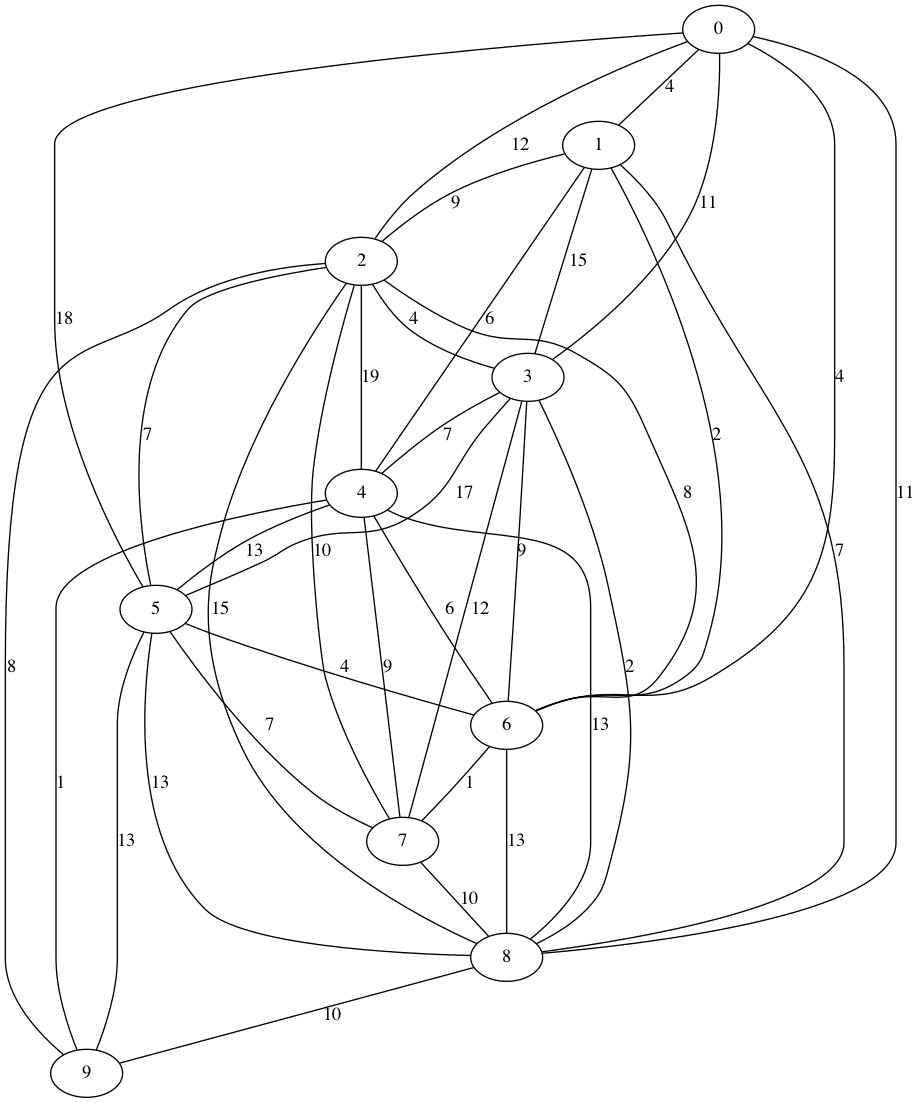
\includegraphics[scale=0.25]{Figures/10_dataset}
	\vspace{1mm}
	\caption{Grafo no dirigido de 10 nodos.}
	\label{grafo_1}
\end{figure}

Después de la partición inicial obtenemos los conjuntos: A = \{3, 4, 6, 8, 9\} y B = \{0, 1, 2 , 5, 7\}.

Los conjuntos tienen el mismo tamaño. Están ordenados.

\section{Spectral Bisection}\label{Spectral-Bisection}

\subsection{Descripción}

\subsection{Ejemplo}

El grafo de ejemplo inicialmente,

\renewcommand{\figurename}{Figura}
\begin{figure}[h]
	\centering
	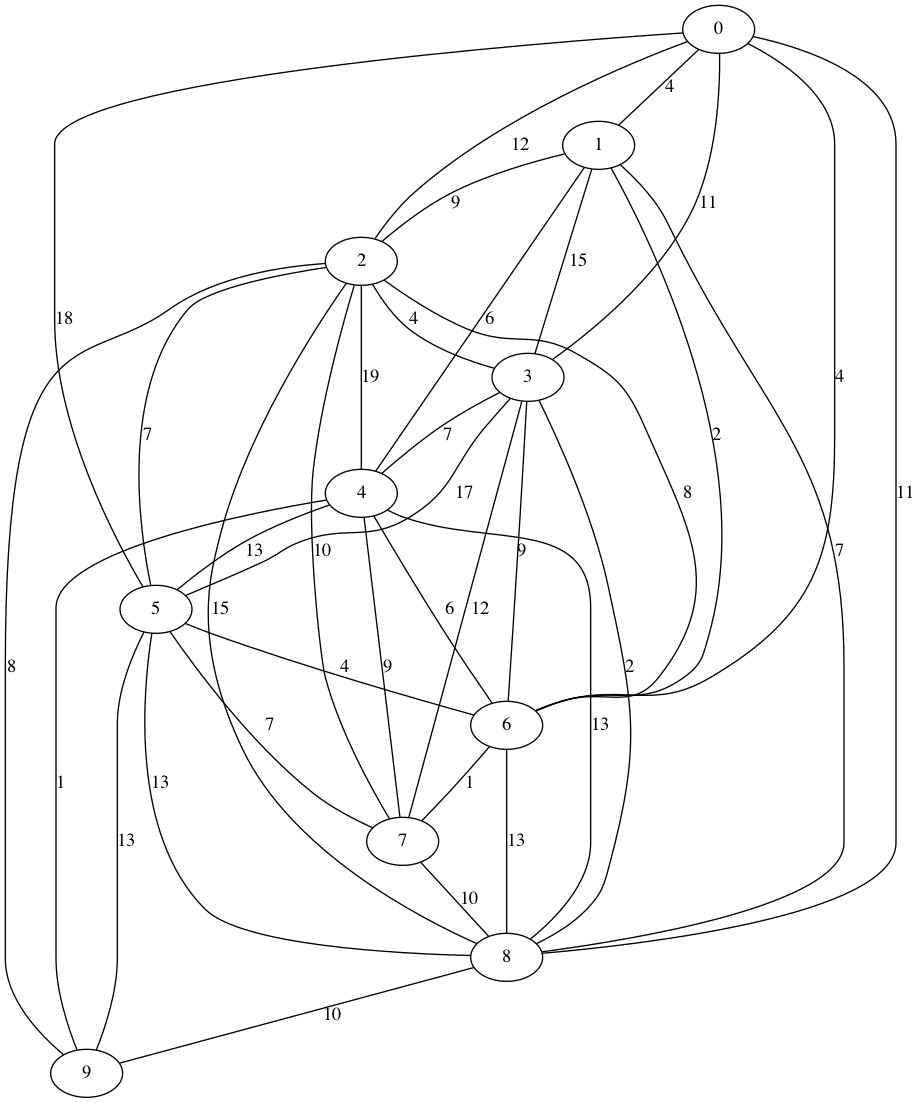
\includegraphics[scale=0.25]{Figures/10_dataset}
	\vspace{1mm}
	\caption{Grafo no dirigido de 10 nodos.}
	\label{grafo_2}
\end{figure}

Después de la partición obtenemos los conjuntos: A = \{1, 2, 3, 4, 6, 9\} y B = \{0, 8, 5, 7\}.

Los conjuntos tienen no son del mismo tamaño. No están ordenados.

\section{Multilevel Spectral Bisection}\label{Multilevel-Spectral-Bisection}

El particionamiento de grafos por multilevel es un método moderno que reduce el tamaño de las particiones del grafo con la combinación de los vértices y las aristas sobre varios niveles, creando particiones del grafo cada vez más pequeñas y extensas con muchas variaciones y combinaciones de diferentes métodos.

METIS es un algoritmo de partición que se enfoca en minimizar el número de bordes de partición cruzados y distribuir la carga de trabajo de manera uniforme entre las particiones. Con METIS, los gráficos se dividen en tres fases. La primera fase es la fase de engrosamiento, la segunda la fase de partición y la tercera y última fase la fase de no engrosamiento (Figura X). La fase de particionamiento contiene particiones bi-particionadas y K-way. A diferencia de la partición K-way, la bi-partición se realiza de forma recursiva. Las subseccion a continuación contienen una explicación más extensa de estas diversas fases.

\subsection{Descripción}

\subsection{Ejemplo}

El grafo de ejemplo inicialmente, vemos que sigue siendo el mismo que en el primer ejemplo (ver Figura \ref{grafo_2}).

\renewcommand{\figurename}{Figura}
\begin{figure}[h]
	\centering
	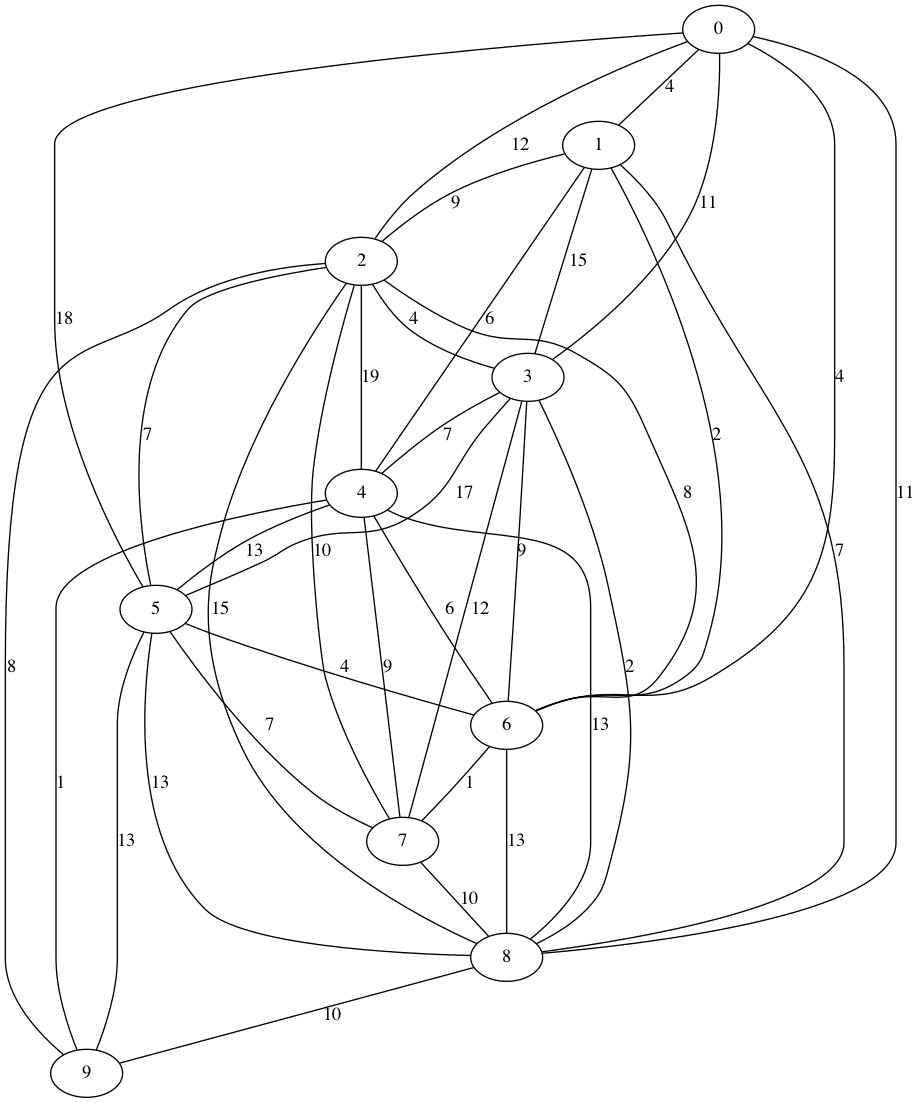
\includegraphics[scale=0.25]{Figures/10_dataset}
	\vspace{1mm}
	\caption{Grafo no dirigido de 10 nodos.}
	\label{grafo_3}
\end{figure}

Después de la partición obtenemos los conjuntos: A = \{0, 1, 3, 7, 8\} y B = \{2, 4, 5, 6, 9\}.

Los conjuntos tienen el mismo tamaño. Están ordenados.